\section{位置、位移与运动模型}
\subsection{质点模型与参考系}
运动学描述物体在哪里、怎样运动，不直接讨论运动改变的原因。能否把物体看成质点取决于所问的问题。研究汽车在两城之间的行程时，车长通常可以忽略；研究汽车能否通过狭窄通道时，车长、车宽和朝向就必须保留。物体尺寸很小并不自动保证质点模型适用，物体尺寸很大也不自动排除这一模型。将运动物体简化为质点以后，仍要明确研究的是车头、质心还是其他代表点。

参考系是描述位置变化所依据的物体或物体组，坐标系是附着于参考系的数学工具。先选参考系，再规定原点、坐标正向和计时起点，才能给坐标的正负以确定意义。同一列车中的旅客相对车厢静止，相对站台却在运动；这不矛盾，因为两个结论的参照不同。更换坐标原点只改变位置数值，更换参考系则可能改变速度。解答中不能把一个参考系的位移与另一个参考系的时间测量条件混用。


图\ref{k1deep:train}明确了质点近似是否适用的判断对象。若求“车头从桥头到桥尾”的时间，只追踪车头坐标即可；若求“整列车完全通过桥”的时间，终态应是车尾到达桥尾，车头实际前进 $L+\ell$，不能只用桥长 $L$。
\fig{k1deep:train}{同一列车，所问事件不同，需要保留的几何长度也不同}{\begin{tikzpicture}[scale=.8]
\draw[thick](0,0)--(7,0);\draw[very thick](2,-.1)--(6,-.1);\node[below]at(2,-.1){桥头};\node[below]at(6,-.1){桥尾};
\draw[fill=blue!12](.4,.15)rectangle(2,.7);\node[above]at(1.2,.7){初态};\node[right]at(2,.4){车头};
\draw[thick](0,-2)--(9,-2);\draw[very thick](2,-2.1)--(6,-2.1);\draw[fill=red!12](6,-1.85)rectangle(7.6,-1.3);\node[above]at(6.8,-1.3){末态};\node[left]at(6,-1.6){车尾};
\draw[guide](2,.7)--(2,1.35) (7.6,-1.3)--(7.6,1.35);\draw[dim](2,1.15)--(7.6,1.15)node[midway,above]{$L+\ell$};
\draw[dim](2,-2.7)--(6,-2.7)node[midway,below]{$L$};\draw[dim](6,-2.7)--(7.6,-2.7)node[midway,below]{$\ell$};
\end{tikzpicture}}
图中追踪的始终是同一个车头，初末态通过车长联系起来。若车速恒为 $u$，整列通过的历时是 $(L+\ell)/u$；若车速变化，仍保留这段位移，只是改用相应运动关系求时间。能否忽略尺寸由所求事件决定，不能仅凭列车相对桥“看起来很小”作判断。


\subsection{位矢、位移与路程}
在固定的平面直角坐标系中，位矢为 $\bm r=x\bm e_x+y\bm e_y$。从位置 $P_1$ 运动到 $P_2$，位移是 $\Delta\bm r=\bm r_2-\bm r_1$，它由起终点确定；路程 $s$ 是沿实际轨迹累积的长度，必须知道中间怎样运动。图\ref{k1theory-path}中，弯曲实线是轨迹，直箭头是位移，两者表示不同的几何对象。
\fig{k1theory-path}{轨迹长度与起终点之间的位移}{\begin{tikzpicture}
\draw[axis](0,0)--(5.6,0)node[right]{$x$};\draw[axis](0,0)--(0,2.8)node[above]{$y$};
\draw[world](.7,.7)..controls(1.2,2.8)and(3.2,2.5)..(4.7,1.3);
\draw[flow,blue](.7,.7)--(4.7,1.3)node[midway,below]{$\Delta\bm r$};
\fill(.7,.7)circle(1.3pt)node[below]{$P_1$};\fill(4.7,1.3)circle(1.3pt)node[right]{$P_2$};
\node at(2.5,2.5){路程沿轨迹累积};\end{tikzpicture}}
因此总有 $s\ge|\Delta\bm r|$，等号要求沿连接两点的直线单向运动。回到出发点时位移为零，路程仍可非零。一维运动中的坐标差 $\Delta x$ 带正负，路程不能带负号；若物体往返，应在每个转向时刻分段，累加各段位移的绝对值。把路程记为位移大小，只有在已经排除转向后才成立。

\subsection{时刻、时间与测量区间}
时刻描述状态，时间间隔描述过程。“第 $n$秒末”对应时间轴上的一个点，“第 $n$秒内”对应从 $n-1$秒到 $n$秒的一段，而“前 $n$秒”从初始时刻连续取到 $n$秒。读图时应把区间端点明确标到时间轴上。位置、速度是时刻的函数，平均速度与路程则必须附带所考察的区间。

测量所得数值还应与模型尺度对应。计算列车通过桥梁的历时，列车长度参与车头到车尾通过的距离，此时不能把整列车缩成一个点；研究列车在相距很远的两站之间的平均速度，车长往往可以忽略。质点不是“体积很小的物体”的别名，而是所求结果对形状、转动和大小不敏感时采用的近似。同一物体在同一道题的不同阶段，也可能需要不同程度的模型描述。

\subsection{分段过程中的局部时间与连续条件}
设$t=t_1$处运动条件改变，第二段用局部时间$\tau=t-t_1$计算。若改变前速度为$v_1$、位置为$x_1$，第二段恒加速度为$a_2$，则局部初值是$v(0)=v_1$、$x(0)=x_1$。先积分速度变化，再积分位置变化：
\begin{align*}
v-v_1&=\int_0^\tau a_2\dd s=[a_2s]_0^\tau=a_2\tau,\\
x-x_1&=\int_0^\tau(v_1+a_2s)\dd s
=\left[v_1s+\frac{a_2s^2}{2}\right]_0^\tau
=v_1\tau+\frac{a_2\tau^2}{2}.
\end{align*}
最后换回全局时间$t$，得到
\[v(t)=v_1+a_2(t-t_1),\qquad
x(t)=x_1+v_1(t-t_1)+\frac12a_2(t-t_1)^2.\]
$x_1,v_1$由第一段末态求出，不能重新置零。无瞬时冲量时速度连续；加速度却可以在外力改变时跳变。若发生理想碰撞，位置仍连续，速度则按碰撞条件突变。把这些不同的连续性要求先写清，比事后猜图像的连接方式更可靠。

时间坐标原点的平移不改变实际过程。例如反应时间 $T$内汽车匀速，制动段用 $\tau=t-T$，初值就必须是制动开始时的位置 $v_0T$与速度 $v_0$。若在制动段仍直接写 $x=v_0t-at^2/2$，等于把制动提前到了零时刻，所算的安全距离将少掉反应阶段。

图\ref{k1k-localtime}标出相同事件的两个时间读数。第一段结束与第二段开始是同一个物理事件，在全局时间中为 $t_1$，在局部时间中为零。求“第几秒相遇”应最后恢复全局时间；求某阶段持续时间则使用局部时间即可。
\fig{k1k-localtime}{局部时间的零点取在阶段切换事件}{\begin{tikzpicture}
\draw[axis](0,0)--(6.5,0)node[right]{$t$};
\foreach \x/\l in {0/0,2.4/t_1,5.5/t}\draw(\x,-.08)--(\x,.08)node[below]{$\l$};
\draw[axis](2.4,-1.4)--(6.5,-1.4)node[right]{$\tau$};
\draw[guide](2.4,0)--(2.4,-1.4) (5.5,0)--(5.5,-1.4);
\node[below]at(2.4,-1.4){$0$};\node[below]at(5.5,-1.4){$t-t_1$};
\draw[dim](2.4,.6)--(5.5,.6)node[midway,above]{同一段时间};
\end{tikzpicture}}



\section{速度、加速度与变化率}
\subsection{平均量与瞬时量}
在同一时间间隔 $\Delta t>0$ 内，平均速度和平均速率分别定义为 $\overline{\bm v}=\Delta\bm r/\Delta t$、$\overline u=s/\Delta t$。平均速度是矢量，平均速率是标量，通常 $\overline u\ne|\overline{\bm v}|$。它们描述整段运动，不能单凭平均值恢复中间任一时刻的瞬时速度。分段运动的平均速度必须先相加位移与时间，不能无条件取各段速度的算术平均。

当时间间隔趋于零，割线趋近轨迹切线，得到
\begin{equation}\bm v=\frac{\dd\bm r}{\dd t},\qquad u=|\bm v|=\frac{\dd s}{\dd t}.\label{eq:k1velocity}\end{equation}
式\eqref{eq:k1velocity}中 $s$ 随运动累积，故 $\dd s/\dd t\ge0$；一维坐标 $x$ 却可以减小。速度方向由瞬时位移的极限给出，在光滑轨迹上沿切线。所谓“经过某位置的速度”还需指定运动分支，同一位置在往返过程中可以对应相反的速度。

\subsection{分段平均为什么需要权重}
设物体沿同一正方向依次走过 $s_1,s_2$，各段速率为 $u_1,u_2>0$。总时间必须逐段相加，因此
\[\overline u=\frac{s_1+s_2}{s_1/u_1+s_2/u_2}.
\]
若给的是各段时间 $t_1,t_2$，同一式又写成 $\overline u=(u_1t_1+u_2t_2)/(t_1+t_2)$。等时间运动取算术平均，等路程运动取调和平均；差别来自统计权重，并非两套彼此无关的技巧。较慢一段占用时间更长，所以等路程的平均速率更偏向较小速率。由 $(u_1-u_2)^2\ge0$还可检验调和平均不超过算术平均。

若包含反向运动，求平均速度时应将 $s_i$改为带符号位移，而求平均速率仍将路程正值相加。以两段等时、大小相等而方向相反的速度为例，平均速度为零，平均速率却保持该速度大小。先写“总位移除总时间”或“总路程除总时间”的定义，可以避免在不同问法之间机械套平均公式。


图\ref{k1deep:average}取两段路程都为 $d$、第一段速率是第二段两倍的情形。空间上的两段一样长，时间轴上的两段却为 $t_0$ 和 $2t_0$，所以整个三份时间中有两份在较慢速度下度过。按时间权重计算，
\[
 \overline u=\frac{(2u)t_0+u(2t_0)}{3t_0}=\frac43u,
\]
而直接平均两个速率会给出 $3u/2$，对应的是另一种“各运动相同时间”的过程。
\fig{k1deep:average}{等路程并不等时间，慢段在平均值中占更大时间权重}{\begin{tikzpicture}
\draw[thick](0,0)--(6,0);\fill(0,0)circle(1.5pt);\fill(3,0)circle(1.5pt);\fill(6,0)circle(1.5pt);
\draw[dim](0,.5)--(3,.5)node[midway,above]{$d$};\draw[dim](3,.5)--(6,.5)node[midway,above]{$d$};
\node[below]at(1.5,0){$2u$};\node[below]at(4.5,0){$u$};
\draw[axis](0,-1.8)--(6.5,-1.8)node[right]{$t$};\fill[blue!20](0,-1.8)rectangle(2,-1.2);\fill[red!20](2,-1.8)rectangle(6,-1.2);
\node at(1,-1.5){$t_0$};\node at(4,-1.5){$2t_0$};\node[below]at(0,-1.8){$0$};\node[below]at(6,-1.8){$3t_0$};
\end{tikzpicture}}


\subsection{矢量变化与加速度}
加速度定义为 $\bm a=\dd\bm v/\dd t$。求速度变化量时，必须先把初、末速度移到同一起点，再作矢量差。图\ref{k1theory-dv}的红箭头从 $\bm v_1$ 的端点指向 $\bm v_2$ 的端点，表示 $\Delta\bm v$；它一般既不平行于初速度，也不平行于末速度。
\fig{k1theory-dv}{速度方向变化本身也产生加速度}{\begin{tikzpicture}
\coordinate(O)at(0,0);\coordinate(A)at(3,0);\coordinate(B)at(2.4,1.8);
\draw[flow](O)--(A)node[midway,below]{$\bm v_1$};\draw[flow,blue](O)--(B)node[midway,above left]{$\bm v_2$};\draw[flow,red](A)--(B)node[midway,right]{$\Delta\bm v$};\node[below left]at(O){$O$};\end{tikzpicture}}
速率不变只能说明速度大小不变，不能说明速度矢量不变。匀速圆周运动便有非零加速度。一维运动中，应以 $va$ 的正负判断速率增减：$va>0$ 时速率增加，$va<0$ 时速率减少；仅说“加速度为负，所以减速”是不充分的。在 $v=0$ 的瞬间，前后是否转向还要检查邻近时刻的速度符号。

\subsection{速率变化与转向的局部判断}
在速度非零的光滑运动段，由 $v^2=\bm v\cdot\bm v$求导，得到
\[2v\dot v=2\bm v\cdot\bm a,\qquad \dot v=\frac{\bm v\cdot\bm a}{v}.\]
这说明加速度在速度方向上的投影控制速率变化，垂直分量则控制方向变化。若某一瞬间点积为零，只能说该瞬间速率变化率为零；要断定一段时间内速率不变，必须证明该条件在整段成立。速度为零时不能再除以 $v$，应回到分量方程分析。

直线运动的转向可用邻近时刻展开检验。若 $v(t_*)=0$且 $a(t_*)\ne0$，则 $v(t_*+\delta t)=a(t_*)\delta t+o(\delta t)$，两侧速度异号，物体在 $t_*$转向。若同时 $a(t_*)=0$，便要检查更高阶项；例如速度正比于 $(t-t_*)^2$时，物体瞬间停下却不转向。因此把“零速度”直接等同于“转折点”会遗漏这一类运动。


图\ref{k1deep:turning}把“过零”和“碰到零点后仍同号”区分开。左图中速度从负到正，位置先减后增，发生转向；右图中速度一直非负，只在 $t_*$ 瞬时为零，位置仍单调增加。需要检查的是零点两侧的速度符号，而不是图线是否碰到了时间轴。
\fig{k1deep:turning}{零速度是转向的候选条件，是否转向取决于两侧符号}{\begin{tikzpicture}[scale=.9]
\begin{scope}\draw[axis](0,0)--(4.1,0)node[right]{$t$};\draw[axis](0,-1.5)--(0,1.9)node[above]{$v$};\draw[blue,thick](.5,-1.2)--(3.5,1.2);\fill(2,0)circle(1.5pt);\node[below right]at(2,0){$t_*$};\node at(2,-2){$v\propto t-t_*$，转向};\end{scope}
\begin{scope}[xshift=5.5cm]\draw[axis](0,0)--(4.1,0)node[right]{$t$};\draw[axis](0,-.4)--(0,1.9)node[above]{$v$};\draw[red,thick,domain=.5:3.5,samples=70]plot(\x,{.6*(\x-2)*(\x-2)});\fill(2,0)circle(1.5pt);\node[below]at(2,0){$t_*$};\node at(2,-2){$v\propto(t-t_*)^2$，不转向};\end{scope}
\end{tikzpicture}}


\subsection{矢量分量与运动方向的交叉核验}
在固定直角坐标系中，$\bm v=(\dot x,\dot y)$、$\bm a=(\ddot x,\ddot y)$。速率为 $v=\sqrt{\dot x^2+\dot y^2}$，对它求导得到
\[\dot v=\frac{1}{2\sqrt{\dot x^2+\dot y^2}}
\bigl(2\dot x\ddot x+2\dot y\ddot y\bigr)
=\frac{\dot x\ddot x+\dot y\ddot y}{v},\qquad v\ne0.\]
这只是加速度沿速度方向的分量。以 $x=A\cos\omega t$、$y=B\sin\omega t$为例，
先对两个位置分量分别求导，再对所得速度分量求导，$A,B,\omega$均保持不变：
\begin{align*}
v_x&=A[-\sin(\omega t)]\omega=-A\omega\sin\omega t,\\
v_y&=B\cos(\omega t)\omega=B\omega\cos\omega t,\\
a_x&=-A\omega\cos(\omega t)\omega=-A\omega^2\cos\omega t,\\
a_y&=B\omega[-\sin(\omega t)]\omega=-B\omega^2\sin\omega t.
\end{align*}
这四个分量合成为$\bm v=\omega(-A\sin\omega t,B\cos\omega t)$、$\bm a=-\omega^2(A\cos\omega t,B\sin\omega t)$。
加速度始终指向原点，但若 $A\ne B$，速率一般不恒定，因为 $v^2=\omega^2(A^2\sin^2\omega t+B^2\cos^2\omega t)$。只有 $A=B$才退化为匀速圆周运动。故“指向固定中心”不足以单独推出匀速，也不足以推出轨迹为圆。

求得分量后，可用三个独立信息检查：位置是否满足轨迹方程，速度是否沿轨迹切线，加速度与速度的点积是否符合速率增减。若某瞬间速度为零，不能使用除以 $v$的式子，应回到位置或速度的局部展开。模型条件、参数范围与特殊点的检验应贯穿整个求解过程。



图\ref{k1deep:ellipse}取 $A>B$ 的椭圆第一象限点。速度沿切线而加速度指向原点，二者一般不垂直；这时加速度同时改变速率和方向。只有在轴端点，或退化成 $A=B$ 的圆时，两者才在图示模型中正交。
\fig{k1deep:ellipse}{指向固定中心的加速度可以包含切向分量}{\begin{tikzpicture}
\draw[axis](-3.4,0)--(3.5,0)node[right]{$x$};\draw[axis](0,-1.8)--(0,2.5)node[above]{$y$};\draw[thick](0,0)ellipse(3 and 1.5);
\coordinate(P)at(2.1213,1.06066);\fill(P)circle(1.7pt)node[right]{$P$};\draw[guide](0,0)--(P);
\draw[force,blue](P)--++(-1.06066,.53033)node[above]{$\bm v$};\draw[force,red](P)--++(-1.2728,-.6364)node[below]{$\bm a$};
\node[below left]at(0,0){$O$};\node[below right]at(3,0){$A$};\node[above left]at(0,1.5){$B$};
\end{tikzpicture}}


\subsection{由运动方程逐次求导}
若 $x(t),y(t)$ 已给出，应在同一时间参数下逐次求导，得到 $v_x=\dot x,v_y=\dot y$，再求 $a_x=\ddot x,a_y=\ddot y$。合速度的大小是 $\sqrt{v_x^2+v_y^2}$，不能把分速度直接相加。加速度的大小同样要由分量合成。消去时间得到轨迹方程后，通常已经丢失了运动快慢，不能仅凭轨迹确定加速度。

反向由速度求位置时，须保留初始条件：$x(t)=x(t_0)+\int_{t_0}^{t}v_x(\tau)\dd\tau$。由加速度积分也先得到速度的变化量，而不是自动得到速度本身。分段函数的交界处应检查位置连续；没有瞬间碰撞或速度突变装置时，速度也应连续。对于速度被指定为阶跃函数的理想模型，连接位置图时仍不能画出位置的跳跃。

\section{图像、微元与几何约束}
\subsection{斜率与面积的不同作用}
$x$--$t$ 图的斜率为速度，$v$--$t$ 图的斜率为加速度；$v$--$t$ 图与时间轴之间的有向面积为位移，绝对面积之和为路程。图线在时间轴下方表示速度为负，不能把其面积在计算位移时仍取正。位置图上的一条水平线表示静止，速度图上的水平线则表示匀速，读图必须先看轴名。

\fig{k1theory-area}{速度图中正负面积共同决定位移}{\begin{tikzpicture}[x=.9cm,y=.65cm]
\draw[axis](0,0)--(6.4,0)node[right]{$t$};\draw[axis](0,-1.5)--(0,2.5)node[above]{$v$};
\fill[blue!12](0,0)--(0,2)--(2,2)--(4,0)--cycle;\fill[red!12](4,0)--(5,-1)--(6,-1)--(6,0)--cycle;
\draw[world](0,2)--(2,2)--(5,-1)--(6,-1);\node at(1.5,.8){$S_+$};\node at(5.4,-.5){$S_-$};\end{tikzpicture}}
图\ref{k1theory-area}中，用 $S_+,S_-$ 表示两块面积的正数值，则 $\Delta x=S_+-S_-$，$s=S_++S_-$。同一组面积可同时给出两个答案。图线斜率突变只意味着加速度改变；速度图中竖直的跳跃才意味着理想化的瞬时速度改变。

\subsection{同一运动怎样在三种图像之间转换}
位置图的纵坐标是位置，速度图的纵坐标是位置变化率，加速度图又是速度变化率。三张图的纵轴量纲不同，同一段斜线不能直接从一张图复制到另一张图。若给定 $v(t)=v_0-at$、$a>0$，以 $x(0)=0$为初值，积分得
\[x(t)=\int_0^t(v_0-a\tau)\dd\tau
=\left[v_0\tau-\frac a2\tau^2\right]_0^t
=v_0t-\frac12at^2.\]
在 $t_*=v_0/a$，速度为零，位置图的斜率也为零；此时 $x_*=v_0^2/(2a)$。若物体继续按同一加速度运动，$t>t_*$时速度变负、位置减小，位置图经过最大值后回落。如果题目说“刹车直到停下”，却应在停下后改为 $v=0$、$x=x_*$，不能把匀减速公式继续外推为倒车。

图\ref{k1k-threegraphs}把两种过程放在同一时间尺度下比较。蓝色实线表示刹停后保持静止，虚线表示同一负加速度继续作用。是否延续虚线由物理条件决定，而不是由已写出的多项式决定。求路程时，前者停后不再增加，后者则继续增加，虽然其带符号位移正在减小。
\fig{k1k-threegraphs}{持续负加速度与刹停后静止对应不同的后续图像}{\begin{tikzpicture}[x=1.2cm,y=1cm]
\begin{scope}
\draw[axis](0,0)--(3.6,0)node[right]{$t$};\draw[axis](0,-.9)--(0,2.4)node[above]{$v$};
\draw[blue,world](0,2)--(2,0)--(3.2,0);
\draw[blue,dashed](2,0)--(2.8,-.8);\node[below]at(2,0){$t_*$};
\end{scope}
\begin{scope}[xshift=6cm]
\draw[axis](0,0)--(3.6,0)node[right]{$t$};\draw[axis](0,0)--(0,2.6)node[above]{$x$};
\draw[blue,world]plot[domain=0:2,samples=40]({\x},{2*\x-.5*(\x)^2});
\draw[blue,world](2,2)--(3.2,2);
\draw[blue,dashed]plot[domain=2:3.2,samples=30]({\x},{2*\x-.5*(\x)^2});
\draw[guide](2,0)--(2,2);\node[below]at(2,0){$t_*$};\node[left]at(0,2){$x_*$};
\end{scope}
\end{tikzpicture}}

由速度图积分位置时，初始位置是必不可少的常数。两物体速度图完全相同，只能推出它们的位移增量相同，不能推出位置相同。反过来，位置图相差一个常量，对应相同的速度图；速度图相差一个常量，则对应相同的加速度图。这些常量分别由最初的位置差和速度差决定。



\subsection{速度随位置变化时怎样累积时间}
若单向运动满足 $v=v(x)>0$，应把每一小段的用时写成 $\dd t=\dd x/v(x)$，于是 $t_2-t_1=\int_{x_1}^{x_2}\dd x/v(x)$。这个积分是 $1/v$--$x$ 图下的面积，不是 $v$--$x$ 图下的面积。量纲也能直接区分：$(1/v)\dd x$ 的单位为时间，$v\dd x$ 的单位却是长度平方除以时间。

微元不是把有限量直接当作零，而是先建立小段关系，再取极限累积。若 $v$ 在端点趋于零，积分可能有限，也可能发散，需要检查趋零方式。发生转向时 $x$ 不再是全程单调参数，应先分支。几何约束题也可使用同一思路：先写每一时刻都成立的长度或位置关系，再对同一个时间求导。

\fig{fv:k1:time}{一小段位移的用时对应倒速度图下的窄条面积}{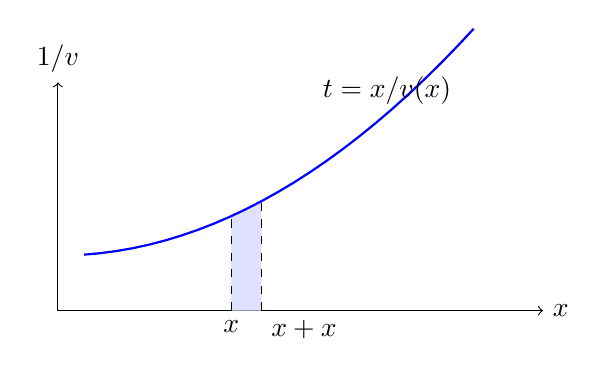
\begin{tikzpicture}[x=1.1cm,y=1cm]
\draw[->](0,0)--(5.6,0)node[right]{$x$};\draw[->](0,0)--(0,2.9)node[above]{$1/v$};
\fill[blue!12](2,0)--(2,1.2)--(2.35,1.39)--(2.35,0)--cycle;
\draw[blue,thick,domain=.3:4.8]plot(\x,{.7+.125*\x*\x});
\draw[dashed](2,0)--(2,1.2);\draw[dashed](2.35,0)--(2.35,1.39);
\node[below]at(2,0){$x$};\node[below right]at(2.35,0){$x+\dd x$};
\node at(3.8,2.8){$\dd t=\dd x/v(x)$};\end{tikzpicture}}
图\ref{fv:k1:time}中的横向小段仍是实际位移，纵向高度却是倒速度。因此低速区域在图上更高，对总用时的贡献更大。若 $v(x)$在某点趋零，不能只看路程有限就认定用时有限，应检查倒速度积分是否收敛。图示只覆盖 $v>0$的单调运动段；发生反向后，应另分一段并按实际方向计算时间。


\subsection{微元近似必须说明被忽略的量}
在足够光滑的运动段，时间增量 $h$内的位置变化为
\[\bm r(t+h)-\bm r(t)=\bm v(t)h+\frac12\bm a(t)h^2+o(h^2).\]
把一小段路程近似为 $v(t)h$时，省略的是更高阶变化。若把总时间分成 $N$段、每段长 $h=T/N$，且每段误差的大小不超过 $Ch^2$，总误差不超过 $NCh^2=CT^2/N$，随 $N$增大趋零。这解释了微小近似为何能在取极限后给出精确积分，而不是因为“每一段看起来都很小”就可以任意相加。

对速度随高度变化的问题，应先写 $\dd t=\dd h/v(h)$。每一段高度的时间权重是速度倒数，不能把 $v$对高度的积分当作时间。若速度依赖时间，累积位移则是 $\int v(t)\dd t$。两个式子的自变量和被积量不同，判断的依据始终是微元的实际意义与量纲。

图\ref{k1k-elements}的等宽高度条在较慢处对应较长的时间条。即使总高度固定，慢区仍可能主导总用时。若接近终点时速度趋零，还应检查积分是否收敛；只有计算出的积分有限，才能说物体在有限时刻到达终点。
\fig{k1k-elements}{等高度微元的时间权重由速度倒数决定}{\begin{tikzpicture}
\draw[axis](0,0)--(5.2,0)node[right]{$h$};\draw[axis](0,0)--(0,2.7)node[above]{$1/v(h)$};
\draw[world](0,.7)--(4.5,2.2);
\fill[blue!20](1,0)rectangle(1.3,1.033333);\fill[red!15](3.5,0)rectangle(3.8,1.866667);
\node[below]at(1.15,0){$\dd h$};\node[below]at(3.65,0){$\dd h$};
\node[above]at(2.3,2.6){条形面积为 $\dd t$};
\end{tikzpicture}}



\subsection{轨迹与时间规律分别确定什么}
若轨迹给成 $\bm r=\bm R(q)$，其中 $q$只是参数而非时间，则链式法则给出
\begin{align*}
\bm v&=\frac{\dd\bm R}{\dd q}\frac{\dd q}{\dd t}=\bm R'(q)\dot q,\\
\bm a&=\frac{\dd}{\dd t}\bigl[\bm R'(q)\dot q\bigr]
=\bigl[\bm R''(q)\dot q\bigr]\dot q+\bm R'(q)\ddot q\\
&=\bm R''(q)\dot q^{\,2}+\bm R'(q)\ddot q.
\end{align*}
第一式中，$\bm R'$决定切线，$\dot q$决定通过的快慢及方向。第二式包含因路径弯曲产生的项和因参数速度变化产生的项。同一轨迹采用不同的 $q(t)$，速度和加速度通常都不同。只有轨迹方程而没有时间条件时，题目对运动的描述尚不完整。

对直线位置函数也可作反向检查。先由给定速度积分再代入初始位置，可以恢复唯一的位置函数；若少给一个初始值，便留有任意常数。加速度需要两个初值才能确定直线运动。求出一个函数只是建立模型的一部分，还应将它求导代回已知条件，并检查所取时间区间内的位置是否越过墙、杆端或其他边界。

在用位置参数积分时间时，端点的可达性尤其容易被忽略。若接近 $x_*$时速率满足 $u\sim C|x_*-x|^p$，$C>0$、$p>0$，取剩余距离 $\xi=|x_*-x|$，时间积分的收敛性由 $\int_0^\varepsilon \xi^{-p}\dd\xi$ 决定。先截去奇点附近 $0<\xi<\delta$，再计算
\[
 \int_\delta^\varepsilon \xi^{-p}\dd\xi
 =\begin{cases}
 [\xi^{1-p}/(1-p)]_\delta^\varepsilon
 =\dfrac{\varepsilon^{1-p}-\delta^{1-p}}{1-p},&p\ne1,\\[4pt]
 [\ln\xi]_\delta^\varepsilon=\ln(\varepsilon/\delta),&p=1.
 \end{cases}
\]
令 $\delta\downarrow0$，$p<1$时 $\delta^{1-p}\to0$，积分有限；$p>1$时 $\delta^{1-p}\to\infty$，连同负分母使积分趋于正无穷；$p=1$的对数也趋于正无穷。因此速度都趋于零，仍可能分别对应有限时刻停住和无限接近而永不到达，必须由趋零规律判断。

\subsection{几何交点与物质点}
两根移动直线的交点、两圆的交点、光斑和影子的位置都能随时间变化，但不一定存在一个物体始终占据这个位置。交点的速度由几何方程决定，不能强令它等于任一条杆上某个物质点的速度。接触约束只要求相对速度在禁止穿透的法线方向分量为零；允许滑动时，切向分量可以不同。

设约束为 $F(x,y,t)=0$，对时间求导得到 $F_x\dot x+F_y\dot y+F_t=0$。式中显含时间的项表示边界本身在运动。若需要加速度，还须再次求导，并保留速度平方产生的项。只把速度关系中的 $v$ 换成 $a$，一般不能得到正确的加速度关系。

\subsection{转动基矢为什么也要求导}
极坐标用距离$\rho$和方位角$\theta$描述位置，径向单位矢量$\bm e_\rho=(\cos\theta,\sin\theta)$，横向单位矢量$\bm e_\theta=(-\sin\theta,\cos\theta)$。它们的长度恒为1，但方向随$\theta(t)$改变。对每个三角函数分量使用链式法则，
\begin{align*}
\dot{\bm e}_\rho&=(-\sin\theta\,\dot\theta,\cos\theta\,\dot\theta)
=\dot\theta\bm e_\theta,\\
\dot{\bm e}_\theta&=(-\cos\theta\,\dot\theta,-\sin\theta\,\dot\theta)
=-\dot\theta\bm e_\rho.
\end{align*}
因此$\bm r=\rho\bm e_\rho$的导数要同时改变长度与方向：$\bm v=\dot\rho\bm e_\rho+\rho\dot{\bm e}_\rho=\dot\rho\bm e_\rho+\rho\dot\theta\bm e_\theta$。

这里的 $\rho\dot\theta$ 是横向分速度，不是一般轨迹的总速率。只有 $\dot\rho=0$ 时，速率才等于 $\rho|\dot\theta|$。继续求加速度时，既要对分量求导，也要对基矢求导；这一规则在圆周运动、转杆及曲线运动中会反复出现。极坐标在 $\rho=0$ 处方位角不确定，经过原点的运动宜改用直角坐标或分段描述。
\subsection{由图像估算与检查量纲}
若速度只以离散测量点给出，可把时间划成小段，用每段平均高度乘宽度估算位移，再逐步缩小步长检查结果是否稳定。曲线过零处应分段，求路程时将负面积取绝对值。位置图的折点表示速度可能突变，速度图的折点表示加速度改变；不要把两类折点理解成同一种物理事件。

量纲检查能排除部分错误：速度应为长度除时间，加速度应为长度除时间平方，角度的弧度数在这些关系中视为无量纲。量纲正确仍只是必要条件，方向、端点和极限检验不可省略；尤其两个三角函数的比值即使量纲相同，也可能因角度定义错误而互为倒数。

\subsection{极坐标加速度的完整展开}
在前述基矢求导关系中令 $\omega=\dot\theta$，直接对速度的两个乘积求导：
\begin{align*}
\frac{\dd}{\dd t}(\dot\rho\bm e_\rho)
 &=\ddot\rho\bm e_\rho+\dot\rho\omega\bm e_\theta,\\
\frac{\dd}{\dd t}(\rho\omega\bm e_\theta)
 &=(\dot\rho\omega+\rho\dot\omega)\bm e_\theta-\rho\omega^2\bm e_\rho.
\end{align*}
两式相加才得到 $a_\rho=\ddot\rho-\rho\omega^2$、$a_\theta=2\dot\rho\omega+\rho\dot\omega$。横向的系数2来自两个不同乘积，而不是需要额外记忆的修正。径向分速度为零并不自动消去径向加速度；固定半径圆周运动正有 $a_\rho=-\rho\omega^2$。

图\ref{k1t-polar-coach}中，$\bm e_\theta$沿角度增加方向，两个相邻径向基矢之差趋向横向。若 $\omega=0$且方向在一段时间内固定，公式退化为沿射线的直线运动；若 $\rho$恒定，则恢复变速圆周运动。这些退化情形同时检查了负号与系数。极坐标的“径向”指相对所选原点，并不总是轨迹的法向，二者只在特殊轨迹上重合。
\fig{k1t-polar-coach}{相邻径向基矢的转动与横向正方向}{\begin{tikzpicture}
\coordinate(O)at(0,0);\coordinate(P)at(2.6,1.5);
\draw[axis](-.3,0)--(4.3,0)node[right]{$x$};
\draw[flow,blue](O)--(P)node[midway,above left]{$\rho\bm e_\rho$};
\draw[guide](O)--(2.15,2.1);
\draw[flow,red](P)--(2,2.54)node[above]{$\bm e_\theta$};
\draw[flow,blue](P)--(3.64,2.1)node[right]{$\bm e_\rho$};
\draw[->](1.2,0)arc(0:30:1.2)node[midway,right]{$\theta$};
\node[below left]at(O){$O$};\node[below right]at(P){$P$};
\end{tikzpicture}}

% thirty-k1-theory
